%//==============================--@--===========================//%
\clearpage
\subsection[5.5 Link-Layer Switches]{\hspace*{0.075 em}\raisebox{0.2 em}{$\pmb{\drsh}$} Link-Layer Switches}
\label{subsec:switches}

\begin{quote}
    ``The role of the switch is to receive incoming link-layer frames and forward them onto outgoing links"\cite{Kurose2017}
\end{quote}

\noindent The switch is \textbf{transparent} to the hosts and routers in the subnet, that is, a host/router addresses a frame to another host/router (rather than addressing the frame to the switch) and happily sends the frame into the LAN, unaware that a switch will be receiving the frame and forwarding it. Switches may also encounter congestion (the rate at which frames arrive to any one of the switch’s output interfaces may temporarily exceed the link capacity of that interface), for which \textbf{they also possess buffers} capable of storing queued frames.

\vspace{1em}
\noindent Both routers and switches are \textbf{store-and-forward devices} with different functionalities:
\begin{itemize}[noitemsep, nolistsep]
    \item \textbf{Routers (encaminhadores):}
    \begin{itemize}[noitemsep, nolistsep]
        \item Operate at the \underline{network layer}.
        \item Determine optimal paths to destinations.
        \item Require configuration.
        \item Protect against broadcast storms.
    \end{itemize}

    \vspace{0.25em}
    \item \textbf{Switches (comutadores):}
    \begin{itemize}[noitemsep, nolistsep]
        \item Operate at the \underline{data link layer}.
        \item Determine a spanning tree for all destinations.
        \item Do not require configuration (plug-and-play).
        \item Do not protect against broadcast storms.
    \end{itemize}
\end{itemize}

%//==============================--@--===========================//%
\subsubsection[5.5.1 Filtering and Forwarding]{$\rightarrow$ Filtering and Forwarding}

\begin{itemize}
    \item \textbf{Filtering:} the switch function that determines if a frame should be forwarded or dropped.
    
    \item \textbf{Forwarding:} the switch function that identifies the interfaces to which a frame should be directed, and moves the frame to those interfaces (switches forward packets based on MAC addresses rather than on IP addresses).
\end{itemize}

\vspace{-1em}
\begin{figure}[H]
    \centering
    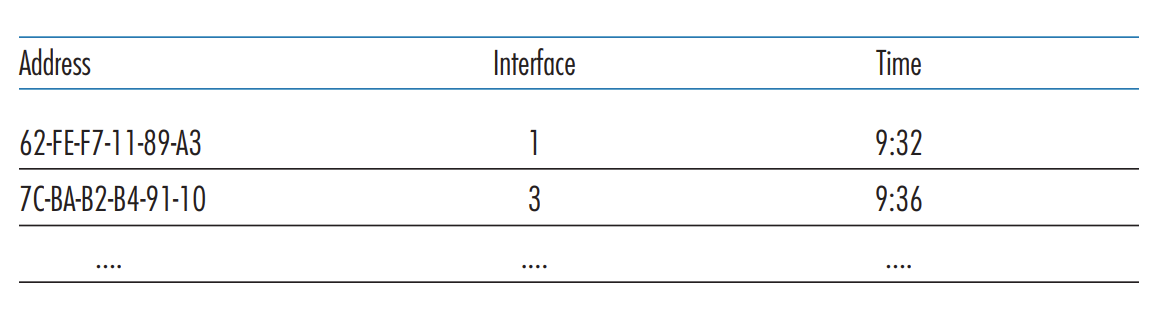
\includegraphics[width = 0.9\linewidth]{img/5/switch-table.png}
    \caption{Portion of a switch table}
    \label{fig:switch-table}
\end{figure}

\vspace{-0.25em}
\noindent Filtering and forwarding actions may take one of the following scenarios:
\begin{enumerate}
    \item \textbf{No table entry for destination address}: Switch broadcasts the frame to all interfaces except the input interface.
    
    \item \textbf{Table entry associates destination with input interface}: Switch filters and discards the frame, as it doesn't need forwarding.
    
    \item \textbf{Table entry associates destination with different output interface}: Switch forwards the frame to the specified output interface.
\end{enumerate}

\begin{figure}[H]
    \centering
    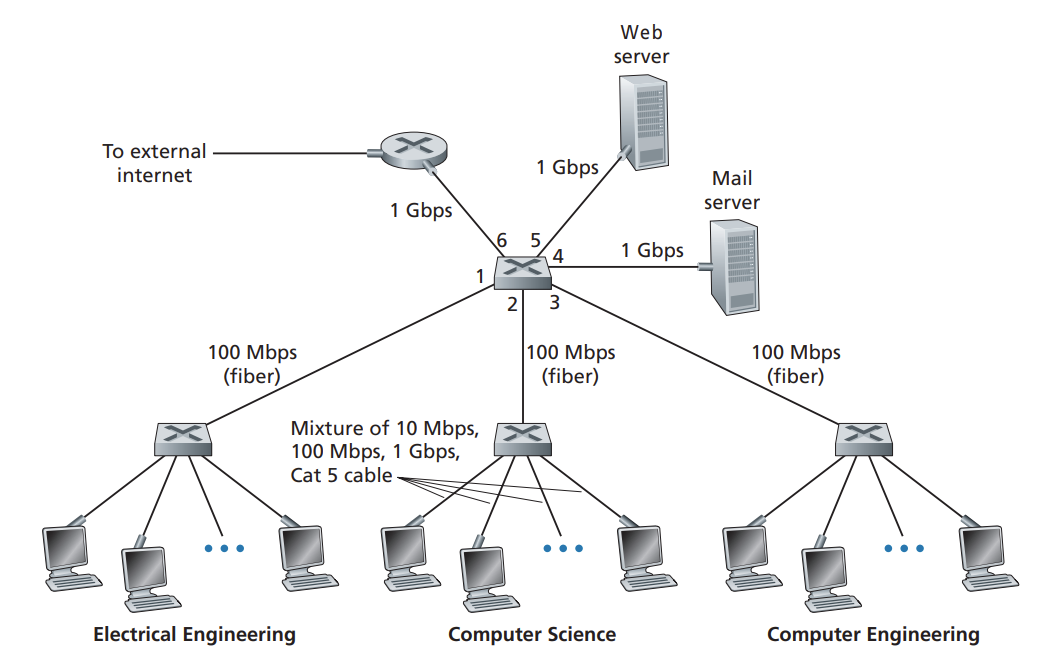
\includegraphics[width = 0.85\linewidth]{img/5/switch-action.png}
    \caption{Diagram of an example subnet}
    \label{fig:switch-action}
\end{figure}

\noindent Taking into account the picture above:
\begin{itemize}
    \item Frame with destination address \texttt{62-FE-F7-11-89-A3} arrives at switch from interface 1: Switch filters (discards) the frame, as it has already been broadcast on the LAN segment containing the destination.
    
    \item Frame with destination address \texttt{62-FE-F7-11-89-A3} arrives from interface 2: Switch forwards the frame to the output buffer preceding interface 1, as the destination is in that direction.
    \item A complete and accurate switch table ensures frame forwarding without unnecessary broadcasting.
\end{itemize}

%//==============================--@--===========================//%
\subsubsection[5.5.2 Self-Learning]{$\rightarrow$ Self-Learning}

\begin{enumerate}
    \item The switch table is initially empty.

    \item For each incoming frame received on an interface, the switch stores the MAC address in the frame's source address field, the interface from which the frame arrived, and the current time. This way, the switch records the LAN segment on which the sender resides.
    
    \item The switch deletes an address in the table if no frames are received with that address as the source address after some period of time (the aging time). This ensures that outdated MAC addresses are eventually purged from the switch table.
\end{enumerate}

\noindent Taking \hyperref[fig:switch-action]{Fig. 56} into consideration again:

\begin{quote}
     ``Suppose at time 9:39 a frame with source address \texttt{01-12-23-34-45-56} arrives from interface 2. Suppose that this address is not in the switch table. Then the switch adds a new entry to the table. Continuing with this same example, suppose that the aging time for this switch is 60 minutes, and no frames with source address \texttt{62-FE-F7-11-89-A3} arrive to the switch between 9:32 and 10:32. Then at time 10:32, the switch removes this address from its table.''\cite{Kurose2017}
\end{quote}

%//==============================--@--===========================//%
\clearpage
\subsubsection[5.5.2 Spanning Tree Protocol (STP)]{$\rightarrow$ Spanning Tree Protocol (STP)}

\noindent The Spanning Tree Protocol (STP) is a link-layer protocol that ensures a loop-free topology in Ethernet networks by creating a spanning tree. It is particularly useful in bridged and switched networks, where loops can cause broadcast storms and result in duplicate frames. STP was standardized as IEEE 802.1D.

\vspace{0.5 em}
\noindent The primary objectives of STP are:
\begin{itemize}[noitemsep, nolistsep]
    \item Preventing loops in the network.
    \item Selecting a designated port for forwarding frames.
    \item Blocking other redundant ports to maintain a loop-free topology.
\end{itemize}

\vspace{0.25 em}
\begin{mdframed}
    \noindent \textbf{STP operates in the following steps:}
    \begin{enumerate}
        \item Elect a root bridge by comparing Bridge IDs (BIDs) which consist of a bridge's priority value and MAC address.
        \item Calculate the shortest path from each switch to the root bridge using path costs.
        \item Select the port with the lowest path cost as the root port for each non-root bridge.
        \item Elect designated ports on each network segment, selecting the port with the lowest path cost to the root bridge.
        \item Block all other ports, putting them in a backup state, preventing loops.
    \end{enumerate}
\end{mdframed}

\noindent During the operation of STP, switches exchange Bridge Protocol Data Units (BPDUs) to share information about network topology and maintain the correct spanning tree state.

\begin{theo}[\underline{Bridge Protocol Data Unit (BPDU)}]{def:BPDU}\label{def:BPDU}
    \noindent BPDUs are special data packets that contain crucial information such as the switch's unique identifier, the sender's root bridge identifier, the sender's root path cost, and the sender's switch port identifier. BPDUs are used by STP to determine the best loop-free topology.
\end{theo}

\begin{figure}[H]
    \centering
    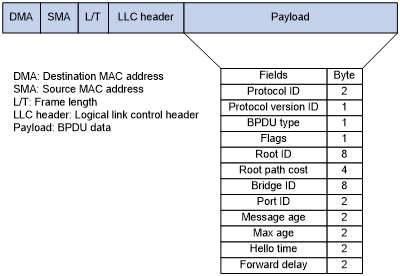
\includegraphics[width = 0.7\linewidth]{img/5/STP-header.png}
    \caption{STP header $[$\textbf{?}$]$}
    \label{fig:STP-header}
\end{figure}

%//==============================--@--===========================//%